\documentclass[a4paper, 14pt]{extreport}
\usepackage{cmap} % для кодировки шрифтов в pdf
\usepackage[T2A]{fontenc} % кодировка с переносами
\usepackage[utf8]{inputenc} %кодировка шрифта
\usepackage[english,russian]{babel} %многоязычность
\usepackage{indentfirst} % отделять первую строку раздела абзацным отступом тоже
\usepackage{pscyr}
\usepackage{ulem} % подчеркивания
\linespread{1.5} %полуторный интервал
\usepackage{setspace}
\setstretch{1.03992} 

\frenchspacing



\usepackage[]{graphicx}
\usepackage[usenames,dvipsnames]{color} % названия цветов
\usepackage{amssymb,amsfonts,amsmath,amsthm,mathtext,cite,enumerate,float} %подключаем нужные пакеты расширений

\usepackage[font=small,labelfont=bf]{caption} 


% \usepackage{makecell}
\usepackage{multirow} % улучшенное форматирование таблиц

\usepackage[unicode, pdftex,pdfpagelabels,bookmarks,hyperindex,hyperfigures]{hyperref} % подключаем hyperref (для ссылок внутри  pdf)

\usepackage{geometry} % Меняем поля страницы
\geometry{left=3cm}% левое поле
\geometry{right=1cm}% правое поле
\geometry{top=2cm}% верхнее поле
\geometry{bottom=2cm}% нижнее поле

\graphicspath{{images/}}

% оглавление
\usepackage{tocloft}
\renewcommand{\cfttoctitlefont}{\hspace{0.38\textwidth} \bfseries\MakeUppercase}
\renewcommand{\cftbeforetoctitleskip}{-1em}
\renewcommand{\cftaftertoctitle}{\mbox{}\hfill \\ \mbox{}\hfill{\footnotesize}\vspace{-2.5em}}
\renewcommand{\cftchapfont}{\normalsize\bfseries \MakeUppercase{\chaptername} }
\renewcommand{\cftsecfont}{\hspace{31pt}}
\renewcommand{\cftsubsecfont}{\hspace{11pt}}
\renewcommand{\cftbeforechapskip}{1em}
\renewcommand{\cftparskip}{-1mm}
\renewcommand{\cftdotsep}{1}
\setcounter{tocdepth}{2}

% стиль библиографии
\usepackage[round,numbers,sort&compress]{natbib}
\renewcommand{\bibnumfmt}[1]{#1.\hfill} % нумерация источников в самом списке — через точку
\renewcommand{\bibsection}{\likechapter{Список использованных источников}} % заголовок специального раздела

\newcommand{\empline}{\mbox{}\newline}
\newcommand{\likechapterheading}[1]{
	\begin{center}
		\textbf{\MakeUppercase{#1}}
	\end{center}
	}
\makeatletter
\renewcommand{\@dotsep}{2}
\newcommand{\l@likechapter}[2]{{\bfseries\@dottedtocline{0}{0pt}{0pt}{#1}{#2}}}
\makeatother
\newcommand{\likechapter}[1]{
	\likechapterheading{#1}
	\addcontentsline{toc}{likechapter}{\MakeUppercase{#1}}}



\usepackage[bf]{titlesec}
\titleformat{\chapter}[display]
{\filcenter}
{\MakeUppercase{\chaptertitlename} \thechapter}
{8pt}
{\bfseries}{}

\titleformat{\section}
{\normalfont\fontsize{16}{16}\bfseries}
{\thesection}
{1em}{}

\titleformat{\subsection}
{\normalsize\bfseries}
{\thesubsection}
{1em}{}

% Настройка вертикальных и горизонтальных отступов
\titlespacing*{\chapter}{0pt}{-36pt}{8pt}
\titlespacing*{\section}{}{*4}{*4}
\titlespacing*{\subsection}{\parindent}{*4}{*4}

\usepackage{lscape} %альбомная ориентация страницы
\usepackage{tikz}
\usepackage{pgfplots}


\usepackage{xcolor,colortbl}
\usepackage{pgf-pie}

\usepackage{xassoccnt}
\NewTotalDocumentCounter{totalfigures}
\NewTotalDocumentCounter{totaltables}
\NewTotalDocumentCounter{totalequations}
\DeclareAssociatedCounters{figure}{totalfigures}
\DeclareAssociatedCounters{table}{totaltables}
\DeclareAssociatedCounters{equation}{totalequations}
\renewcommand{\thetable}{\thechapter.\arabic{table}}
\renewcommand{\thefigure}{\thechapter.\arabic{figure}}
\usepackage{lastpage}
\usepackage{totcount}
\newtotcounter{citenum}
\def\oldcite{}
\let\oldcite=\bibcite
\def\bibcite{\stepcounter{citenum}\oldcite}

\usepackage{pgfplots}
\usepackage{ragged2e}
\usepackage{microtype}

\usepackage{titlesec}
\titleformat{\chapter}[hang] 
{\normalfont\bfseries}{{ГЛАВА }\thechapter}{1em}{}
\usepackage{caption}
\DeclareCaptionLabelFormat{mylabel}{#1 #2 -\hspace{1.5ex}}
\begin{document}
	\def\figurename{Рисунок}
	\def\bibname{СПИСОК ИСПОЛЬЗОВАННОЙ ЛИТЕРАТУРЫ}
	\captionsetup{labelfont={}, justification=centering, labelformat=mylabel,labelsep=none}
	\hypersetup{
		colorlinks=false,
		pdfborder={0 0 0},
	}
	\justifying
	\sloppy
	\tolerance=500
	\hyphenpenalty=10000
	\emergencystretch=3em
	\setlength{\abovedisplayskip}{30pt}
	\setlength{\belowdisplayskip}{30pt}
	\setlength\extrarowheight{10pt}
	\begin{titlepage}
		\linespread{1.1}
		\begin{center}
			\fontsize{14pt}{14pt}\selectfont
			\textbf{МИНЕСТЕРСТВО ОБРАЗОВАНИЯ РЕСПУБЛИИ БЕЛАРУСЬ}\\
			\textbf{БЕЛОРУССКИЙ ГОСУДАРСТВЕННЫЙ УНИВЕРСИТЕТ}\\
			\textbf{ФАКУЛЬТЕТ ПРИКЛАДНОЙ МАТЕМАТИКИ И ИНФОРМАТИКИ}\\
			\textbf{Кафедра вычислительной математики}\\
			\vspace{3.5cm}
			\fontsize{14pt}{14pt}\selectfont
			Стефанович Константин Андреевич\\
			\vspace{1.0cm}
			\textbf{Построение параллельного алгоритма численного решения двумерного уравнения Пуассона на основе красно-черного упорядочивания}\\
			\vspace{1.0cm}
			\fontsize{14pt}{14pt}\selectfont
			Курсовая работа\\
		\end{center}
		\vspace{1.5cm}
		\fontsize{14pt}{14pt}\selectfont
		\hspace{-0.5cm}
		\def\arraystretch{1.2}
		\begin{tabular}{l@{\hspace{5.25cm}}l}
			 &Научный руководитель:\\
			 &доктор физ.-мат. наук,\\
			 &профессор Н.А. Лиходед\\
			Допущен к защите&\\
			<<\underline{~~~~}>>~~\underline{~~~~~~~~~~~~} 2018 г&\\
		\end{tabular}
		\begin{flushleft}
			Зав. кафедрой вычислительной математики,
			кандидат физико-математических наук, доцент В.И. Репников
		\end{flushleft}
	
		\vspace{3.0cm}
		\begin{center}
			\fontsize{14pt}{14pt}\selectfont
			Минск, 2018
		\end{center}
	\end{titlepage}
	\newpage
	\setcounter{page}{2}
	\begin{center}
		\fontsize{16pt}{16pt}\selectfont
		\textbf{РЕФЕРАТ}
	 \end{center}
 	\vspace{1.1cm}

	\textbf{Работа содержит}: \TotalValue{totaltables} таблиц, \TotalValue{totalfigures} рисунков, \pageref{LastPage} страниц, \total{citenum} сайтов,  \TotalValue{totalequations} формул.

	\textbf{Ключевые слова}: ИТЕРАЦИОННЫЕ ПАРАЛЛЕЛЬНЫЕ АЛГОРИТМЫ, КРАСНО-ЧЕРНОЕ УПОРЯДОЧЕНИЕ, OPENMP.
	
	\textbf{Объект исследования} – параллельный алгоритм численного решения двумерного уравнения Пуассона на основе красно-чёрного упорядочения.
	
	\textbf{Цель работы} – исследование параллельного алгоритма на основе красно-чёрного упорядочения, сравнение его с параллельными алгоритмами Якоби и Зейделя.
	
	\textbf{В результате} – разработан и программно реализован параллельный алгоритм на основе красно-чёрного упорядочения.
	
	
	\newpage
	\renewcommand\contentsname{ОГЛАВЛЕНИЕ} 
	\tableofcontents
	\newpage
	

	\begin{center}
		\fontsize{14pt}{14pt}\selectfont
		\textbf{АННОТАЦИЯ}
	\end{center}
	\begin{center}
		на курсовую работу «Построение параллельного алгоритма численного решения двумерного уравнения Пуассона на основе красно-черного упорядочивания»
	\end{center}
	
	
	В данном уравнении исследуется параллельный алгоритм численного решения двумерного уравнения Пуассона на основе красно-чёрного упорядочения. Также будет разработан и программно реализован параллельный алгоритм на основе красно-чёрного упорядочения.

	\newpage
	\likechapter{Введение}
	\vspace{1.1cm}
	
	В математике уравнение Пуассона – это эллиптическое дифференциальное уравнение в частных производных, которое широко применяется на практике (инженерное дело) и теории (теоретическая физика). В частности, оно описывает потенциальное поле, вызванное заданным распределением плотности заряда или массы. Также в физике часто используется уравнение Лапласа, которое является частным случаем уравнения Пуассона. Уравнение названо в честь знаменитого французского математика, геометра и физика Симеона Пуассона(Подробнее смотрите в \citealp{wiki})
	
	Уравнение Пуассона можно представить в виде $ \Delta u = f$, где $\Delta$ – оператор Лапласа, а $f$ и $\varphi$  – вещественные или комплексные функции на некотором многообразии. Обычно функция $f$ нам дана, а функцию $\varphi$ нужно найти. 
	
	В двумерных декартовых координатах уравнение принимает вид (\ref{eq0_1}): 
	\begin{equation}\label{eq0_1} 
		\frac{\partial^2 u}{\partial x_1^2} + \frac{\partial^2 u}{\partial x_2^2} = f(x_1, x_2)
	\end{equation}
	
	Если $f=0$, то уравнение Пуассона превращается в уравнение Лапласа: $\Delta\varphi=0$.
	
	Уравнение Пуассона можно решить явно с помощью функции Грина, существует также много способов численного решения, например, релаксационный метод.
	\chapter{МАТЕМАТИЧЕСКАЯ ПОСТАНОВКА ЗАДАЧИ}
	\vspace{1.1cm}
	\section{Аппроксимация}
	Рассмотрим двумерную задачу Дирихле для уравнения Пуассона (\ref{eq1_1}):
	\begin{equation}\label{eq1_1}
		\begin{cases}
			\frac{\partial^2 u}{\partial x_1^2} + \frac{\partial^2 u}{\partial x_2^2} = f(x_1, x_2); (x_1, x_2) \in G \\
			u(x_1, x_2)|_\Gamma = \mu(x_1, x_2), \\
		\end{cases}
	\end{equation}
	где $G$ - прямоугольная область $[0<x_1<l_1]\times[0<x_2<l_2]$ с границей $\Gamma$.
	
	Пусть нами задана равномерная прямоугольная сетка (\ref{eq1_2}):
	\begin{equation}\label{eq1_2} 
		\{ih_1,i=0,1,\dots,N_{x_1}, N_{x_1}h_1=l_1, jh_2, j=0,1,\dots,N_{x_2}, N_{x_2}h_2=l_2\}
	\end{equation}
	
	Запишем теперь разностную задачу Дирихле на данной сетке, используя пятиточечный шаблон "крест" (Формула (\ref{eq1_3}), рисунок \ref{i1_1}):
	\begin{equation}\label{eq1_3} 
		\begin{cases}
			\frac{u_{i+1,j}-2u_{i,j}+u_{i-1,j}}{h_1^2} + \frac{u_{i,j+1}-2u_{i,j}+u_{i,j-1}}{h_2^2} = f_{ij}, \\
			u|_{\gamma_h} = \mu(x_1, x_2)|_{\gamma_h} \\
			i=0,1,\dots,N_{x_1} ; j=0,1,\dots,N_{x_2} \\
		\end{cases}
	\end{equation}
	где $\gamma_h$ - граничные узлы.
	\begin{figure}[h]
		\begin{center}
			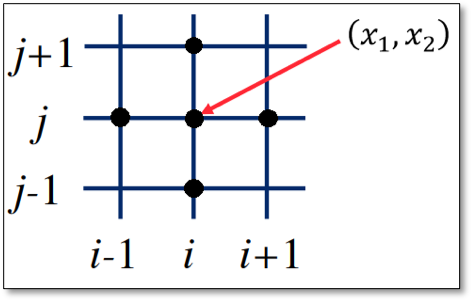
\includegraphics[width=0.5\linewidth]{5_dots}
			\captionof{figure}{Пятиточечный шаблон $''$крест$''$}
			\label{i1_1}
		\end{center}
	\end{figure}

	Записанную систему линейных алгебраических уравнений относительно $u_{ij}$ обычно решают итерационными методами. Перед началом вычислений задают начальное (обычно нулевое) приближение $u^0_{ij}$ во внутренних точках сетки, а значения $u^0_{ij}$ в граничных узлах заполняют точными значениями $\mu_{ij}$.
	
	Рассмотрим несколько итерационных методов.
	
	\subsection{Итерационный процесс Якоби}
	Итерационный процесс метода Якоби имеет следующий вид (\ref{eq1_4}):
	\begin{equation}\label{eq1_4}
		\begin{split}
			u^{k+1}_{i,j} = 
				\left(\frac{2}{h_1^2}+\frac{2}{h_2^2}\right)^{-1} 
				\left(\frac{u_{i+1,j}^k+u_{i-1,j}^k}{h_1^2} + \frac{u_{i,j+1}^k+u_{i,j-1}^k}{h_2^2} - f_{ij}\right)\\
			i=0,1,\dots,N_{x_1}; j=0,1,\dots,N_{x_2}; k=0,1,\dots
		\end{split}
	\end{equation}
	
	Если $h=h_1=h_2$, тогда получаем (\ref{eq1_5}): 
	\begin{equation}\label{eq1_5}
		\begin{split}
			u^{k+1}_{i,j} = \frac{1}{4}
				\left(u_{i+1,j}^k+u_{i-1,j}^k+u_{i,j+1}^k+u_{i,j-1}^k - h^2f_{ij}\right)\\
			i=0,1,\dots,N_{x_1}; j=0,1,\dots,N_{x_2}; k=0,1,\dots
		\end{split}
	\end{equation}
	
	Данный метод не очень часто используется на практике, так как требует дополнительной матрицы, что увеличивает память и время работы программы, так как часть этого времени используется на копирование элементов.
	Подробнее смотрите в \citealp{falechik}, \citealp{estproceses}.
	
	\subsection{Итерационный процесс  Зейделя}
	Итерационный процесс метода Зейделя имеет следующий вид (\ref{eq1_6}):
	\begin{equation}\label{eq1_6}
		\begin{split}
			u^{k+1}_{i,j} = 
				\left(\frac{2}{h_1^2}+\frac{2}{h_2^2}\right)^{-1} 
				\left(\frac{u_{i+1,j}^k+u_{i-1,j}^{k+1}}{h_1^2} + \frac{u_{i,j+1}^k+u_{i,j-1}^{k+1}}{h_2^2} - f_{ij}\right)\\
			i=0,1,\dots,N_{x_1}; j=0,1,\dots,N_{x_2}; k=0,1,\dots
		\end{split}
	\end{equation}
	
	Если $h=h_1=h_2$, тогда получаем (\ref{eq1_7}):
	\begin{equation}\label{eq1_7}
		\begin{split}
			u^{k+1}_{i,j} = \frac{1}{4}
				\left(u_{i+1,j}^k+u_{i-1,j}^{k+1}+u_{i,j+1}^k+u_{i,j-1}^{k+1} - h^2f_{ij}\right)\\
			i=0,1,\dots,N_{x_1}; j=0,1,\dots,N_{x_2}; k=0,1,\dots
		\end{split}
	\end{equation}
	
	Алгоритм Зейделя имеет то преимущество, что в компьютерной реализации нам больше не нужно выделять два массива. Вместо этого мы можем сделать только один массив и выполнять все обновления значений только в нём. Ещё метод Зейделя дает более быстрое уменьшение ошибки, чем метод Якоби.
	Подробнее смотрите в \citealp{eukm}.
	
	\subsection{Итерационный процесс с красно-черным упорядочением}
	
	Рассмотрим способ обхода узлов сетки, который основывается на их «красно-черном» упорядочивании (Рисунок \ref{i1_2}). В соответствии с этим приемом все узлы сетки делятся на два подмножества $\Omega_1$  и $\Omega_2$  (сеточные узлы «раскрашиваются» в черные и красные цвета в шахматном порядке), а поскольку при получении разностных схем использовался шаблон пятиточечный «крест», для расчета значения сеточной функции в узле черного цвета нужны значения в узлах красного цвета и наоборот.
	В этом методе узлы в анализируемом сетке делятся на 2 блока в шахматном порядке. Во время обхода алгоритма все красные точки обновляются до черных точек. Для двумерной задачи Пуассона мы видим, что для обновления красной точки сетки требуется только информация из черных точек сетки и наоборот. Следовательно, порядок, в котором обновляются точки в каждом наборе, не имеет значения. Поскольку блоки разного цвета являются независимыми друг от друга, итерации можно распараллелить для каждого цвета. Аналитическое исследование показывает, что скорость сходимости улучшается за счет увеличения числа узлов одного блока и легко устанавливается оптимальный размер блока для получения наилучшей скорости сходимости. Численные тесты показывают, что метод достигает большого ускорения из-за быстрой конвергенции, небольших затрат синхронизации и эффективного использования кэша данных на скалярном параллельном компьютере.
	
	Подробнее смотрите в \citealp{gergel}, \citealp{hey}.
	\begin{figure}[h]
		\begin{center}
			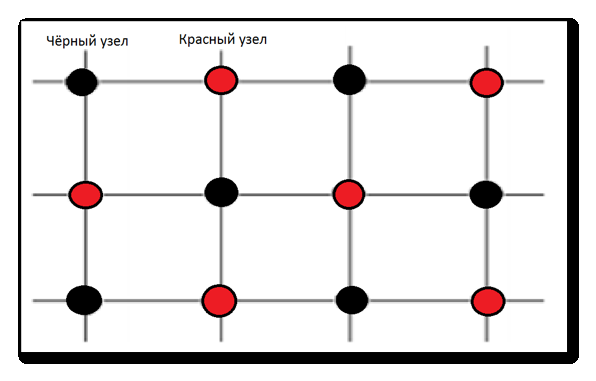
\includegraphics[width=0.5\linewidth]{red-black.eps}
			\captionof{figure}{$''$Красно-черное$''$ упорядочивание узлов сетки(векторное изображение)}
			\label{i1_2}
		\end{center}
	\end{figure}
	\section{Распараллеливание и Open MP}
	Существует множество различных технологий параллельного программирования. Причем эти технологии различаются не столько языками программирования, сколько архитектурными подходами построения параллельных систем. 
	
	Определенные технологии, например, предполагают построение параллельных алгоритмов на одной машине с несколькими процессорными ядрами, другие же – нескольких компьютеров (одного или нескольких типов). 
	
	Системы параллельного программирования для работы на одной машине, начали развиваться не так давно. Не стоит думать, что это принципиально новые идеи, но именно с приходом многоядерных систем на рабочий стол, программистам стоит обратить свое внимание на такие технологии как Open MP, Intel Thread Building Blocks, Microsoft Parallel Extensions и ряд других.
	
	Очень важно, чтобы технология параллельного программирования поддерживала возможность делать введение параллельности в программу постепенно. Идеальную параллельную программу стоит с самого начала писать параллельной, предпочтительнее, используя какой-либо функциональный язык, где не стоит вопрос распараллеливания как таковой. Однако в реальном мире, где вместо функционального $F\#$ есть 10 Мбайт кода на C++, и такой код надо постепенно распараллеливать. В таком случае технология Open MP (например) является довольно удачным решением, т.к. она позволяет, выделив в приложении приоритетно нуждающиеся в параллелизации места, начать распараллеливание именно их. Как это выглядит на практике – с помощью какого-то инструмента профилирования программист находит в программе «узкие места», которые замедляют работу программы, затем эти программист распараллеливает их с помощью Open MP, после чего, можно искать следующие узкие места и так, до тех пор, пока не будет получена желаемая производительность. Именно такой подход сделал технологию Open MP довольно популярной.
	
	Open MP (Open Multi-Processing) – это набор директив компилятора, переменных окружения и библиотечных процедур, предназначенных для программирования многопоточных программ на многопроцессорных системах с общей памятью (SMP-системах).
Подробнее смотрите в \citealp{fpmi}, \citealp{anton}
	
	Первый стандарт Open MP был разработан в 1997 г. как ориентированный на написание легко переносимых многопоточных приложений API. Сначала он был основан на Fortran, но позднее включил в себя С и С++.
	
	Интерфейс Open MP стал крайне популярной технологией параллельного программирования и успешно используется как для программирования суперкомпьютерных систем с множеством процессоров, так и в настольных пользовательских системах.
	
	Над спецификацией Open MP ведет работу множество крупных производителей вычислительной техники и ПО, чья работа регулируется некоммерческой организацией «Open MP Architecture Review Board» (ARB).
	
	В Open MP используется модель параллельного выполнения «ветвление-слияние» (Рисунок \ref{i1_3}) – программа начинается как единый поток выполнения, называемый начальным. При встрече потоком параллельной конструкции, происходит создание новой группы потоков, состоящей из начального и некоторого числа дополнительных потоков, где начальный поток остается главным. Все члены новообразованной группы (включая главный) выполняют код внутри параллельной области. В конце параллельной области есть неявный барьер, после которого выполнение пользовательского кода продолжает только главный поток. В параллельную конструкцию могут быть вложены и другие параллельные конструкции, в которых каждый поток изначального региона становится основным для своей новой группы потоков. Вложенные регионы могут в свою очередь включать регионы еще более глубокого уровня вложенности.
	\begin{figure}[h]
		\begin{center}
			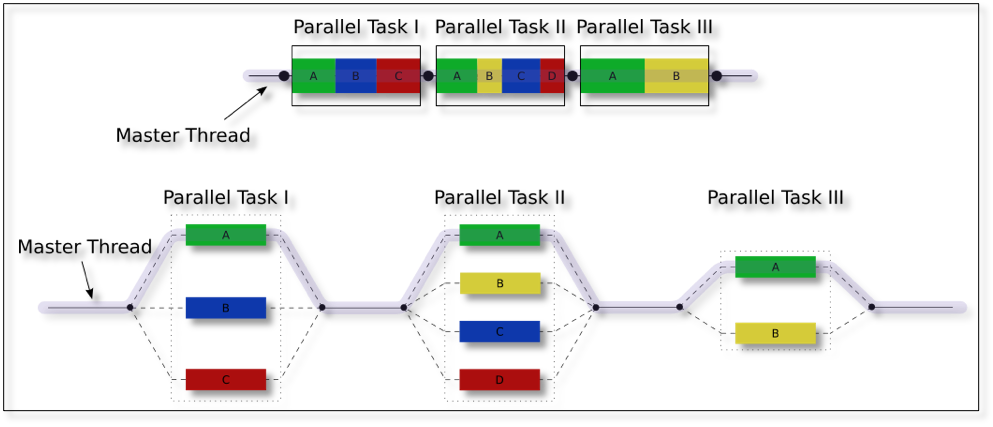
\includegraphics[width=\linewidth]{openmp}
			\captionof{figure}{Схематическое изображение модели параллельного исполнения Open MP}
			\label{i1_3}
		\end{center}
	\end{figure}
	Число потоков в группе, выполняющихся параллельно, можно контролировать несколькими способами. Один из них – использование переменной окружения OMP\_NUM\_THREADS. Другой способ – вызов процедуры omp\_set\_num\_threads(). Еще один способ – использование выражения num\_threads в сочетании с директивой parallel.
	
	В Open MP существует ряд вспомогательных функций. Для их использования не забудьте подключить заголовочный файл <omp.h>.
	
	\subsection{Функции исполняющей среды}
	Эти функции позволяют запрашивать и задавать различные параметры среды Open MP:
	\begin{itemize}
		\item omp\_get\_num\_procs – возвращает число вычислительных узлов (процессоров/ядер) в компьютере;
		\item omp\_in\_parallel – позволяет потоку узнать, занимается ли он в данный момент выполнением параллельного региона;
		\item 	omp\_get\_num\_threads – возвращает число потоков, входящих в текущую группу потоков;
		\item 	omp\_set\_num\_thread – задает число потоков для выполнения следующего параллельного региона, который встретится текущему выполняемому потоку. Функция может помочь распределить ресурсы. Например, если мы одновременно обрабатываем звук и видео на процессоре с четырьмя ядрами, то можно создать для звука один поток, а для обработки видео –три;
		\item 	omp\_get\_max\_threads – возвращает максимально допустимое число нитей для использования в следующей параллельной области;
		\item 	omp\_set\_nested – разрешает или запрещает вложенный параллелизм. Если вложенный параллелизм разрешён, то каждая нить, в которой встретится описание параллельной области, породит для её выполнения новую группу нитей и станет в ней главной;
		\item 	omp\_get\_nested – возвращает, разрешен ли вложенный параллелизм или нет.
	\end{itemize}

	Если имя функции начинается с omp\_set\_, то ее можно вызывать только вне параллельных регионов. Все остальные функции можно использовать как внутри параллельных регионов, так и вне таковых.
	
	\subsection{Функции синхронизации/блокировки}
	Open MP позволяет строить параллельный код без использования этих функций, так как имеются директивы, позволяющие осуществлять определенные виды синхронизации. Однако в ряде случаев эти функции удобны и даже необходимы.
	
	В Open MP два типа блокировок: простые и вложенные. Вложенные имеют суффикс «nest». Блокировки могут находиться в одном из трех состояний – неинициализированном, заблокированном и разблокированном.
	\begin{itemize}
		\item omp\_init\_lock/omp\_init\_nest\_lock – инициализация переменной типа omp\_lock\_t/omp\_nest\_lock\_t. Аналог InitializeCriticalSection.
		\item	omp\_destroy\_lock/omp\_destroy\_nest\_lock – освобождение переменной типа omp\_lock\_t/omp\_nest\_lock\_t. Аналог DeleteCriticalSection.
		\item	omp\_set\_lock/omp\_set\_nest\_lock – один поток выставляет блокировку, а остальные потоки ждут, пока поток, вызвавшая эту функцию, не снимет блокировку с помощью функции omp\_unset\_lock(). Аналог EnterCriticalSection.
		\item	omp\_unset\_lock/omp\_unset\_nest\_lock – снятие блокировки. Аналог LeaveCriticalSection.
		\item	omp\_test\_lock/omp\_test\_nest\_lock – неблокирующая попытка захвата замка. Данная функция пробует захватить указанный замок. Если это удалось, то для простого замка функция возвращает 1. Если замок захватить не удалось, то возвращается 0. Аналог TryEnterCriticalSection.
	\end{itemize}
	
	Простые блокировки (omp\_lock\_t) не могут быть установлены более одного раза, даже тем же потоком. Вкладываемые блокировки (omp\_nest\_lock\_t) идентичны простым с тем исключением, что когда поток пытается установить уже принадлежащую ему вкладываемую блокировку, он не блокируется.
	
	\subsection{Функции работы с таймерами }
	\begin{itemize}
		\item omp\_get\_wtime – возвращает в вызвавшем потоке астрономическое время в секундах (вещественное число двойной точности - double), прошедшее с некоторого момента в прошлом. Если некоторый участок программы окружить вызовами данной функции, то разность возвращаемых значений покажет время работы данного участка.
		\item omp\_get\_wtick () – возвращает в вызвавшем потоке разрешающую  способность таймера в секундах, то есть точность таймера
		\item if (условие) – выполнение параллельной области по условию. Создание нескольких потоков осуществляется только при выполнении некоторого условия. Если условие не выполнено, то код выполняется в последовательном режиме.
		\item num\_threads – явное задание количества потоков, которые будут выполнять параллельную область. По умолчанию выбирается последнее значение, установленное с помощью функции omp\_set\_num\_threads().
	\end{itemize}


	\newpage
	\chapter{ПРАКТИЧЕСКАЯ РЕАЛИЗАЦИЯ ЗАДАЧИ }
	\section{Точечный параллельный алгоритм, выполняющий заданное число итераций. }
	Будем находить решение следующей задачи (\ref{eq2_1}):
	\begin{equation}\label{eq2_1} 
		\begin{cases}
			\frac{\partial^2 u}{\partial x_1^2} + \frac{\partial^2 u}{\partial x_2^2} = 2e^{x_1+x_2}; (x_1, x_2) \in [0<x_1<1]\times[0<x_2<1] \\
			u(0, x_2)=e^{x_2}; u(1, x_2)=e^{x_2+1}; u(x_1, 0)=e^{x_1}; u(x_1, 1)=e^{x_1+1}  \\
		\end{cases}
	\end{equation}
	Заметим, что точным решением данной задачи будет являться функция $u(x_1,x_2)=e^{x_1+x_2 }$, график функции изображен на (Рисунок \ref{i2_1})
	\begin{figure}[h]
		\begin{center}
			\begin{tikzpicture}
			\begin{axis}[view/h=-30]
				\addplot3[
					surf,
					shader=flat,
					samples=50,
					domain=-1:1,y domain=-1:1
				] 
					{e^(x+y)};
			\end{axis}
			\end{tikzpicture}
			\captionof{figure}{График точного решения}
			\label{i2_1}
		\end{center}
	\end{figure}

	Вычислительные эксперименты проводились на компьютере с 4-мя ядрами.
	
	Для всех вычислений в этом разделе возьмём шаг $h=0.025$ и три разных значения количества итераций - 10 и 100,1000.
	
	Для удобства на каждом графике изобразим как точное, так и приближенное решение.
	
	Точность решения на определённой итерации можно оценивать разными способами, мы будем использовать следующую формулу:
$\delta = max|u_{i,j}^{n+1} - u_{i,j}^n|$
	
	\subsection{Итерационный процесс Якоби }
	Сначала посмотрим на поведение приближенного решения при 100 итерациях:
	
	Погрешность, подсчитанная по приведённой выше формуле, составляет 0.0195057.
	
	Теперь проведём 1000 итераций (Рисунок \ref{i2_3}):

	На этот раз видим, что приближенное решение почти совпало с точным, а, следовательно, может использоваться на практике. Погрешность составляет уже около 0.00065 $6.5*10^{(-4)})$. Опытным путем также можно показать, что при увеличении количества итераций до 5000 погрешность уменьшается до $2.8*10^{(-9)}$
	
	\begin{figure}[h]
		\begin{center}
			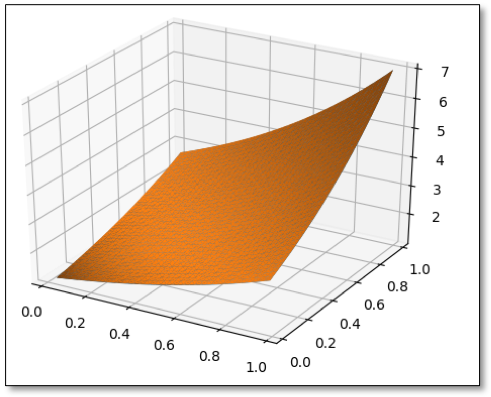
\includegraphics[width=0.5\linewidth]{yacobi_1000}
			\captionof{figure}{График для метода Якоби,  тысяча итераций}
			\label{i2_3}
		\end{center}
	\end{figure}

    \subsection{Итерационный процесс с упорядочением }
    В данном разделе мы рассмотрим алгоритм красно-черного упорядочения на 1, 2, 3, 4 и 8 потоках, также будем менять количество итераций и шаг сетки. Попробуем найти оптимальное количество потоков для решения этой задачи. Количество итераций алгоритма выбиралось так, чтобы погрешность примерно равнялась нулю. Погрешность также будет приведена в результатах работы алгоритма (Таблица \ref{t2_1}, Рисунок \ref{i2_4}, Рисунок \ref{i2_9}).
    
    Формула для подсчёта погрешности:
$\delta = max|u_{i,j}^{n+1} - u_{i,j}^n|$
    
    Каждый вычислительный эксперимент был проведён в количестве 5 раз, в графиках, диаграммах и таблицах приведены средние значения.

    \begin{center}
    	\captionof{table}{h = 0.005, количество итераций = 10.000} \label{t2_1}
    	\begin{tabular}{ | p{0.3\linewidth} | p{0.2\linewidth}  | p{0.2\linewidth} | p{0.2\linewidth} |}
    		\hline
    		Номер эксперимента & Затраченное время (в секундах) & Вычислительная погрешность  \\ \hline
    		1 & 29.190 & 0.000001  \\ \hline
    		2 & 28.520 & 0.000001  \\ \hline
    		3 & 28.420 & 0.000001  \\ \hline
    		4 & 28.430 & 0.000001 \\ \hline
    		5 & 28.470 & 0.000001 \\ \hline
    		Итог & \cellcolor{red!50}28.606 & \cellcolor{green!50}0.000001 \\ \hline
    		1 & 14.700 & 0.000001  \\ \hline
    		2 & 14.350 & 0.000001  \\ \hline
    		3 & 14.480 & 0.000001  \\ \hline
    		4 & 14.470& 0.000001  \\ \hline
    		5 & 14.500 & 0.000001  \\ \hline
    		Итог & 14.500 & \cellcolor{green!50}0.000001 \\ \hline
    		1 & 10.170 & 0.000001  \\ \hline
    		2 & 10.130 & 0.000001  \\ \hline
    		3 & 10.180 & 0.000001  \\ \hline
    		4 & 10.240 & 0.000001  \\ \hline
    		5 & 10.270 & 0.000001  \\ \hline
    	\end{tabular}
     \end{center}
 
	Красная ячейка в таблице обозначает худшее время или погрешность, зелёная – лучшее.

	\begin{center}
		\begin{tikzpicture}
			\begin{axis}[
				enlargelimits=0.15,
				ybar=5pt,
				bar width=9pt,
				nodes near coords
			]
			\addplot
				coordinates {(1,28.6) (2,14.5)
				(3,10.2) (4,8) (5,8.15)};
			\end{axis}
		\end{tikzpicture}
		\captionof{figure}{Диаграмма при h = 0.005, количество итераций = 10.000}
		\label{i2_4}
	\end{center}

	\begin{center}
		\begin{tikzpicture}
		\pie{41/1, 21/2, 15/3, 11/4, 12/5}
		\end{tikzpicture}
		\captionof{figure}{Те же самые данные, но в виде "pie" диаграммы}
		\label{i2_9}
	\end{center}
	
	Приведём сравнение времени выполнения последовательных и параллельных алгоритмов для алгоритмов Зейделя и красно-черного упорядочения.
	
	Отсюда видно, что при большом количестве итераций метод Зейделя становится все менее эффективным.
	
	Из проведенных экспериментов можно сделать следующие выводы:
	\begin{itemize}
		\item Как показали все эксперименты, кроме первого, наилучшее время всегда показывали 4 потока. Это связано с тем, сто программа тестировалась на компьютере с 4-мя ядрами. Это видно, когда мы смотрим на результаты работы программы с 8 потоками – она работает даже чуть больше, чем программа с четырьмя. Это связано с тем, что при большем количестве потоков увеличивается время переключения их между собой. Логические ядра, судя по всему, на время работы программы не влияют.
		\item Для первого эксперимента никакой существенной корреляции между количеством потоков и временем работы программы выявлено не было. Это означает, что при достаточно малом шаге количество потоков перестает влиять на время работы программы.
		\item  Наиболее эффективное количество потоков для работы на большой сетке равно количеству ядер используемого компьютера.
		\item  Среднее ускорение при увеличении количества потоков в 2 раза составило примерно 1.8 – 1.9
		\item  При большой размерности сетки и большом количестве итераций на практике выгоднее использовать метод Красно-черного упорядочения, а не метод Зейделя. В приведенных последовательных алгоритмах при вычислении нового значения y(i, j) используются или значения, полученные на предыдущей итерации (алгоритмы типа Якоби), или вполне конкретные значения, полученные как на предыдущей, так и на текущей итерации (алгоритмы зейделевского типа). При параллельных реализациях возможно использование значений, полученных на предыдущей и на текущей итерации, но не обязательно указанных на какой из них. Такого типа параллельные сеточные алгоритмы называются алгоритмами хаотической релаксации.
Подробнее смотрите в \citealp{gergel}, \citealp{hey}.
	\end{itemize}

	\newpage
	\section{Итерационный процесс с оценкой погрешности}
	В данном разделе мы рассмотрим параллельный алгоритм красно-черного упорядочения на 1, 2, 3, 4, 8 потоках, также будем менять количество итераций и шаг сетки. Вместе с ним мы также рассмотрим эффективность параллельного алгоритма Зейделя и сравним их. Попробуем найти оптимальное количество потоков для решения этой задачи. Формула для расчёта погрешности во всех примерах такая:
$\delta = max|u_{i,j}^{n+1} - u_{i,j}^n|$
	
	Каждый вычислительный эксперимент был проведён 50 раз, в графиках приведены средние значения (Рисунок \ref{i2_6}, \ref{i2_7}, \ref{i2_8}):
	
	\newpage
	
	\begin{figure}[h]
		\begin{center}
			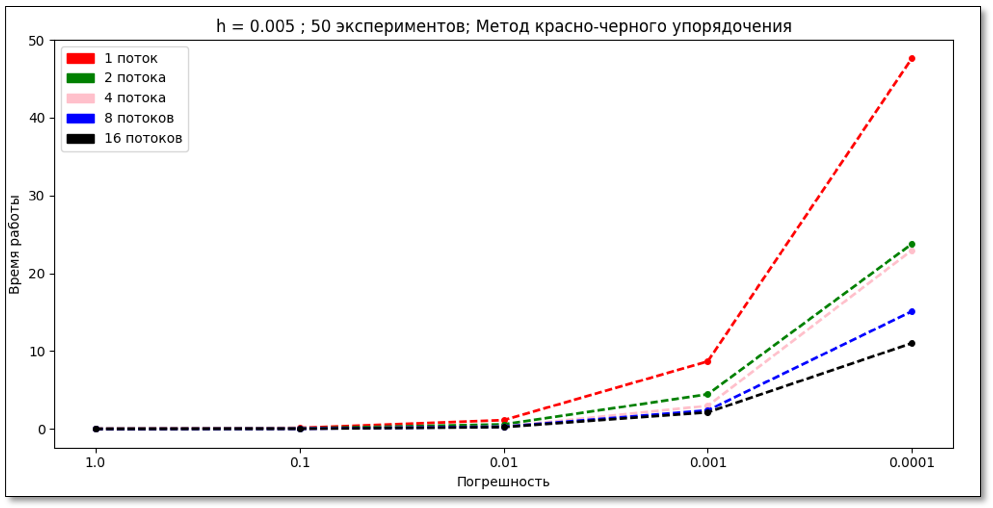
\includegraphics[width=0.7\linewidth]{ch2_1}
			\captionof{figure}{Зависимость времени работы от погрешности и количества потоков (h = 0.005, Метод красно-черного упорядочения)}
			\label{i2_6}
		\end{center}
	\end{figure}
	
	\begin{figure}[h]
		\begin{center}
			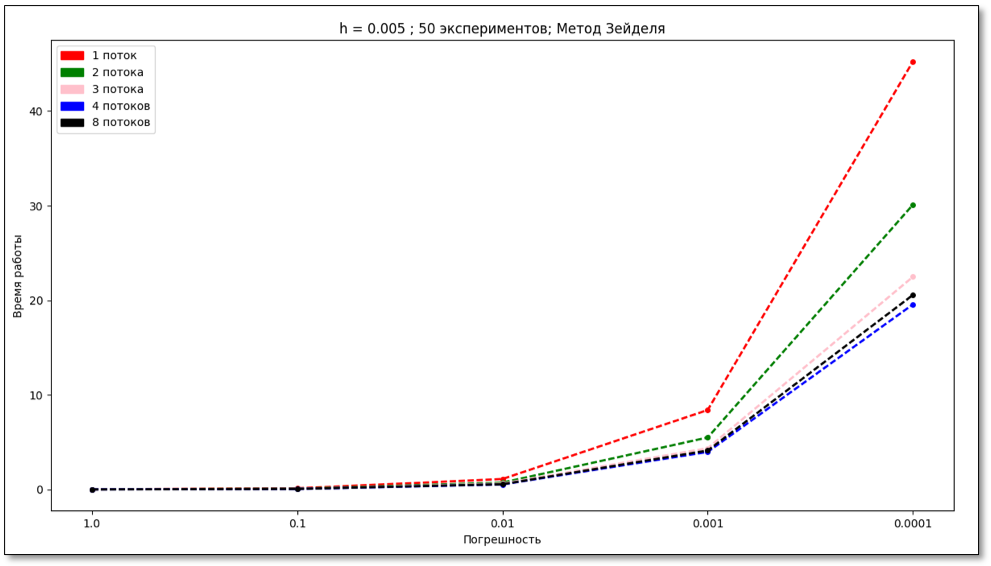
\includegraphics[width=0.7\linewidth]{ch2_2}
			\captionof{figure}{Зависимость времени работы от погрешности и количества потоков (h = 0.005, Метод Зейделя)}
			\label{i2_7}
		\end{center}
	\end{figure}

	\begin{landscape}
		\begin{figure}[h]
			\begin{center}
				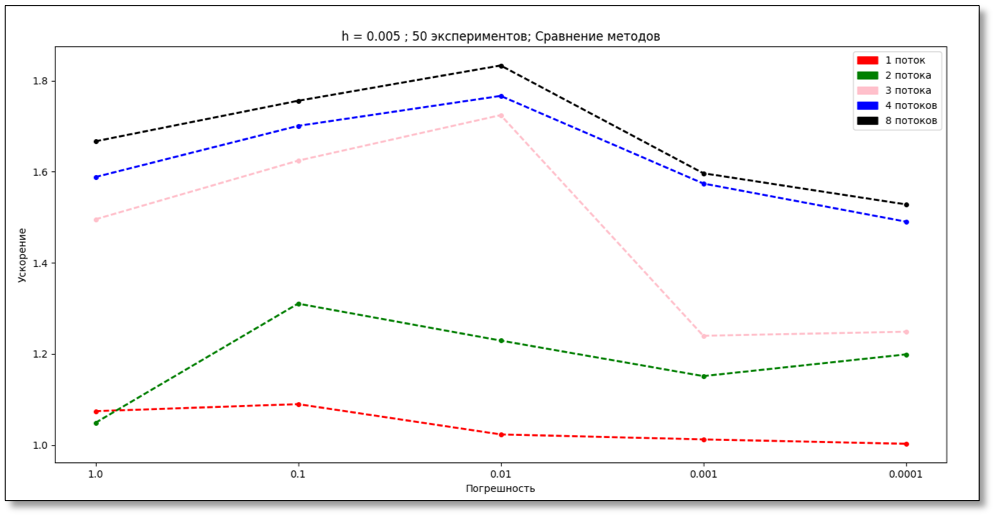
\includegraphics[width=0.9\linewidth]{ch2_3}
				\captionof{figure}{h = 0.005, сравнение ускорения метода Красно-черного упорядочения в сравнении с методом Зейделя при разном количестве потоков и разной погрешности.}
				\label{i2_8}
			\end{center}
		\end{figure}
	\end{landscape}
	
	Из проведенных экспериментов можно сделать следующие выводы:
		\begin{itemize}
		\item В целом все выводы о наилучшем количестве потоков такие же, как и в прошлом разделе – целесообразно использовать количество потоков, равное количеству ядер компьютера.
		\item Ускорение метода красно-черного упорядочения при увеличении количества потоков в 2 раза чуть ухудшилось по сравнению с точечным параллельным алгоритмом и составило 1.7 – 1.8. Это связано с необходимостью подсчитывать погрешность вычислений на каждой итерации алгоритма.
		\item Ускорение метода красно-черного упорядочения по сравнению с методом Зейделя растёт с ростом числа потоков – так, например, для двух потоков оно составило в среднем 1.3, а для четырёх уже 1.65.
	\end{itemize}
	
\newpage
\likechapter{Заключение}
При параллельной реализации метод красно-черного упорядочения особенно эффективен на большом количестве итераций (или на большой сетке и среднем/большом количестве итераций). При использовании пятиточечного шаблона он обладает большой по сравнению с методом Зейделя точностью на любом количестве потоков, что связано с особенностями многопоточной обработки. Для расчётов наиболее рационально использовать количество потоков, равное количеству ядер компьютера, это количество является наиболее эффективным их расчёта потраченой памяти / занятого времени. Также в ходе работы был рассмотрен метод Якоби, который даже по сравнению с методом Зейделя даёт худшее время.

\newpage
\begin{thebibliography}{9}
	\bibitem{falechik} Фалейчик, Б.В. Вычислительные методы алгебры: базовые понятия и алгоритмы : учеб.-метод. пособие / Б. В. Фалейчик. — Минск : БГУ, 2010. — 42 с.
	\bibitem{wiki} Гринин, Л. Е. Социальная макроэволюция: генезис и трансформации Мир-Системы / Л. Е. Гринин, А. В. Коротаев. – Изд. 2-е. – М. : URSS, 2013. – 567 с.
	\bibitem{eukm} Rips, L. J. Lines of thought: central concepts in cognitive psychology / L. J. Rips. – New York ; Oxford : Oxford Univ. Press, 2011. – XXII, 441 p.
	\bibitem{estproceses} Закономерности формирования и совершенствования системы движений спортсменов (на примере метания копья) / В. А. Боровая [и др.]. – Гомель: Гомел. гос. ун-т, 2013. – 173 с.
	\bibitem{gergel} Агапов, Е. П. Методы исследования в социальной работе: учеб. пособие / Е. П. Агапов. – 2-е изд. – М. : Дашков и К° ; Ростов н/Д : Наука-Спектр, 2013. – 223 с.
	\bibitem{hey} Reforming the United Nations for peace and security [Electronic resource]: proc. of a workshop to analyze the rep. of the High-level Panel on Threats, Challenges, a. Change / Yale Center for the Study of Globalization. – New Haven: Yale Center for the Study of Globalization, 2005. – Mode of access:\href{ http://www.ycsg.yale.edu/core/forms/Reforming_un.pdf}{ http://www.ycsg.yale.edu/core/forms/Reforming_un.pdf}
	– Date of access: 20.02.2018.
	\bibitem{anton} Узел крепления крановых рельсов к стальным подкрановым балкам. Технические условия: СТБ 2135-2010. – Введ. 01.07.11 (с отменой на территории РБ ГОСТ 24741-81). – Минск: Белорус. гос. ин-т стандартизации и сертификации, 2011. – 6 с. 
	\bibitem{fpmi} 	Национальный правовой Интернет-портал Республики Беларусь [Веб-сайт]. – Режим доступа: \href{http://www.pravo.by}{http://www.pravo.by}. – Дата доступа: 24.06.2018.
	\bibitem{gost} 	ГОСТ 7.9 – 77. Реферат и аннотация. – М. : Изд-во стандартов, 1981. – 6 с..\right 
\end{thebibliography}
\end{document}